% Editable source for profile.pdf, written by make_profile_figure.py from smoke/profile_local.json
\documentclass[tikz,border=6pt]{standalone}
\usepackage[T1]{fontenc}
\begin{document}
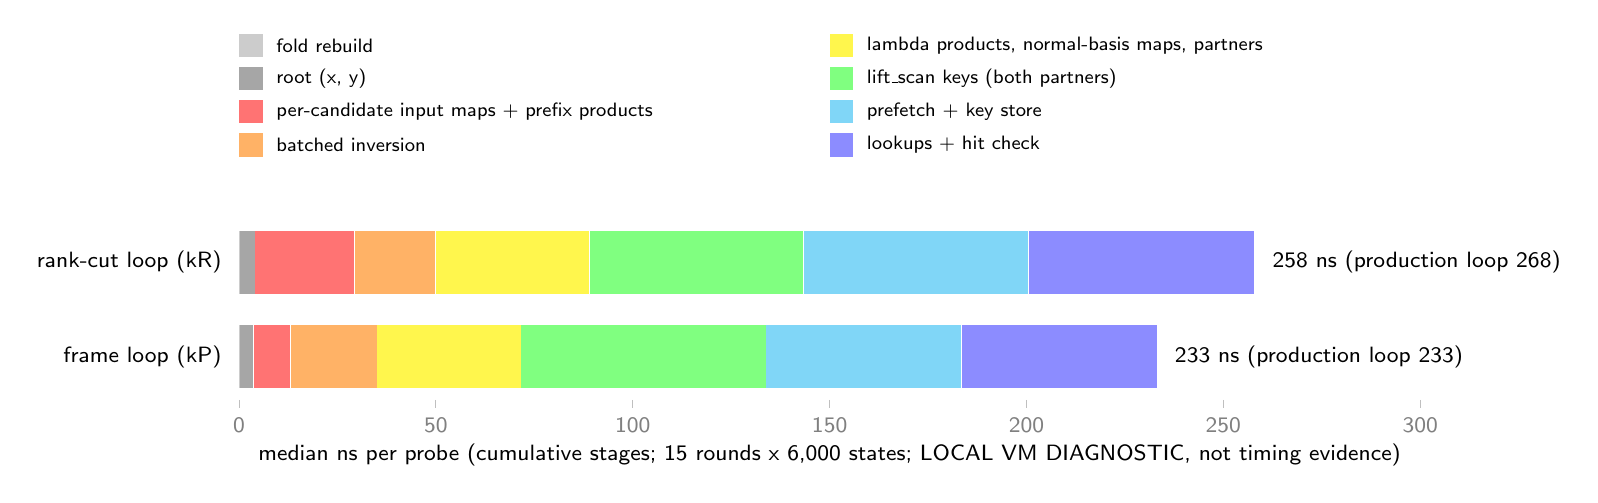
\begin{tikzpicture}[font=\sffamily\footnotesize]
\fill[gray!40] (0.000,-0.40) rectangle (0.017,0.40);
\draw[white] (0.017,-0.40) -- (0.017,0.40);
\fill[gray!70] (0.017,-0.40) rectangle (0.204,0.40);
\draw[white] (0.204,-0.40) -- (0.204,0.40);
\fill[red!55] (0.204,-0.40) rectangle (1.466,0.40);
\draw[white] (1.466,-0.40) -- (1.466,0.40);
\fill[orange!60] (1.466,-0.40) rectangle (2.501,0.40);
\draw[white] (2.501,-0.40) -- (2.501,0.40);
\fill[yellow!70] (2.501,-0.40) rectangle (4.457,0.40);
\draw[white] (4.457,-0.40) -- (4.457,0.40);
\fill[green!50] (4.457,-0.40) rectangle (7.169,0.40);
\draw[white] (7.169,-0.40) -- (7.169,0.40);
\fill[cyan!50] (7.169,-0.40) rectangle (10.027,0.40);
\draw[white] (10.027,-0.40) -- (10.027,0.40);
\fill[blue!45] (10.027,-0.40) rectangle (12.902,0.40);
\draw[white] (12.902,-0.40) -- (12.902,0.40);
\node[anchor=east] at (-0.1,0.00) {rank-cut loop (kR)};
\node[anchor=west] at (13.002,0.00) {258 ns (production loop 268)};
\fill[gray!40] (0.000,-1.60) rectangle (0.017,-0.80);
\draw[white] (0.017,-1.60) -- (0.017,-0.80);
\fill[gray!70] (0.017,-1.60) rectangle (0.190,-0.80);
\draw[white] (0.190,-1.60) -- (0.190,-0.80);
\fill[red!55] (0.190,-1.60) rectangle (0.657,-0.80);
\draw[white] (0.657,-1.60) -- (0.657,-0.80);
\fill[orange!60] (0.657,-1.60) rectangle (1.756,-0.80);
\draw[white] (1.756,-1.60) -- (1.756,-0.80);
\fill[yellow!70] (1.756,-1.60) rectangle (3.582,-0.80);
\draw[white] (3.582,-1.60) -- (3.582,-0.80);
\fill[green!50] (3.582,-1.60) rectangle (6.697,-0.80);
\draw[white] (6.697,-1.60) -- (6.697,-0.80);
\fill[cyan!50] (6.697,-1.60) rectangle (9.180,-0.80);
\draw[white] (9.180,-1.60) -- (9.180,-0.80);
\fill[blue!45] (9.180,-1.60) rectangle (11.662,-0.80);
\draw[white] (11.662,-1.60) -- (11.662,-0.80);
\node[anchor=east] at (-0.1,-1.20) {frame loop (kP)};
\node[anchor=west] at (11.762,-1.20) {233 ns (production loop 233)};
\draw[gray!50] (0.00,-1.75) -- (0.00,-1.85) node[below,gray] {0};
\draw[gray!50] (2.50,-1.75) -- (2.50,-1.85) node[below,gray] {50};
\draw[gray!50] (5.00,-1.75) -- (5.00,-1.85) node[below,gray] {100};
\draw[gray!50] (7.50,-1.75) -- (7.50,-1.85) node[below,gray] {150};
\draw[gray!50] (10.00,-1.75) -- (10.00,-1.85) node[below,gray] {200};
\draw[gray!50] (12.50,-1.75) -- (12.50,-1.85) node[below,gray] {250};
\draw[gray!50] (15.00,-1.75) -- (15.00,-1.85) node[below,gray] {300};
\node at (7.50,-2.45) {median ns per probe (cumulative stages; 15 rounds x 6,000 states; LOCAL VM DIAGNOSTIC, not timing evidence)};
\fill[gray!40] (0.00,2.60) rectangle (0.30,2.90); \node[anchor=west,font=\sffamily\scriptsize] at (0.35,2.75) {fold rebuild};
\fill[gray!70] (0.00,2.18) rectangle (0.30,2.48); \node[anchor=west,font=\sffamily\scriptsize] at (0.35,2.33) {root (x, y)};
\fill[red!55] (0.00,1.76) rectangle (0.30,2.06); \node[anchor=west,font=\sffamily\scriptsize] at (0.35,1.91) {per-candidate input maps + prefix products};
\fill[orange!60] (0.00,1.34) rectangle (0.30,1.64); \node[anchor=west,font=\sffamily\scriptsize] at (0.35,1.49) {batched inversion};
\fill[yellow!70] (7.50,2.60) rectangle (7.80,2.90); \node[anchor=west,font=\sffamily\scriptsize] at (7.85,2.75) {lambda products, normal-basis maps, partners};
\fill[green!50] (7.50,2.18) rectangle (7.80,2.48); \node[anchor=west,font=\sffamily\scriptsize] at (7.85,2.33) {lift\_scan keys (both partners)};
\fill[cyan!50] (7.50,1.76) rectangle (7.80,2.06); \node[anchor=west,font=\sffamily\scriptsize] at (7.85,1.91) {prefetch + key store};
\fill[blue!45] (7.50,1.34) rectangle (7.80,1.64); \node[anchor=west,font=\sffamily\scriptsize] at (7.85,1.49) {lookups + hit check};
\end{tikzpicture}
\end{document}
